\chapter{Programming and Method}\label{chap:prog}
\begin{overview}
  The software developed for this project is described in this chapter.
  Attention is given to the following aspects;
  \begin{itemize}
    \item software design,
    \item programming language,
    \item external tools and
    \item selected code overviews.
  \end{itemize}
\end{overview}

\section{Assumptions}
Certain assumptions are made about the systems investigated.
This serves to define the scope of the project and aids in the mathematical rigour of the methods.
\begin{itemize}
\item Steady-state models are used.
  These models result in real matrices and allow for strictly linear transformation of spaces.
\item Only linear constraints are considered.
  This allows for half-space geometry to be used and ensures convexity of intersections (along with the assumption of steady-state gain models).
\item The convexity of all spaces are assumed.
  This allows the use of minimum vertex descriptions.
\end{itemize}
It should be noted that this is a subset of the available problems.
It is by no means implied that rigorous mathematical methods are only possible for this given subset.

Note that when reference is made to a ``constraint set'', all the half-spaces comprising the set as well as the feasible region (of the set) is implied.

\section{Programming language}
The routines developed for this project was done using the Python programming language.
The SciPy and NumPy modules provide the majority of the mathematical functions used.
The programs were compiled in Linux (Ubuntu 10.4) and this is at present the only supported platform.

\section{Qhull}\label{sec:qhull}
Extensive use is made of the \qhull algorithm \citep{qhull} for the calculation of normals, vertices and hypervolumes.
This algorithm was selected on the basis of its multidimentional functionality and the availability of Unix binaries.
Other Python libraries were considered but deemed insufficient, the most prominent routines being;
\begin{itemize}
\item The \texttt{spatial} module of SciPy contains a Python implementation of the \qhull algorithm but does not currently allow for volume and normal calculation.
\item The CGAL-Python project \citep{cgal} provides Python bindings to the Computational Geometry Algorithms Library (CGAL) but does not more than 3 dimensions.
\end{itemize}

For this project, the \qhull algorithm is directly implemented from its Unix binaries.
A Python subprocess call is used, with communication to/from \qhull by standard input and standard output.
It should be noted that the \qhull algorithm works with vertices and conversion between vertices and half-spaces are done throughout the code.

\section{Constraint set class}
\label{sec:conclass}
A Python class, \texttt{ConSet}, was created to handle constraint sets.
Commonly used attributes of these sets were added as properties of the class and commonly used operations were added as methods.

\subsection{Constructors}
Constraint sets can be constructed from the set of constraints or from the vertices of their feasible region.
For construction from vertices, the set is assumed to be closed and the corresponding constraints are generated accordingly.
Open sets can occur when constructing from constraints as the half-spaces comprising the set are predefined.
Open sets are flagged as erroneous and construction does not proceed.

\subsection{Methods}
The methods of the \texttt{ConSet} class are briefly discussed below.

\subsubsection{Volume}
The \qhull algorithm is used to calculate the hypervolume of the constrain set.
%% MEMOIZE VOLUME and expand

\subsubsection{Space conversion}
The process model is used when converting from the input space to the output space (or vice versa).
When using a steady-state model (real matrix of gains) this results in a matrix multiplication.
Therefore, the output of this operation is a linear transformation of the vertices of the initial constraint set.

It needs to be noted that since the steady-state gain model of the system is used, changes in outputs are the result of the matrix multiplication.
The output values around which the model was linearised are used to translate the output space to absolute values.  

\subsubsection{Intersections}
When the intersection of two constraint sets need to be calculated (as is the case with the AOS and the DOS), a method of superfluous constraints is used.

In an attempt to avoid the problem of degeneracy (section~\ref{sec:hgeometry}) the constraints that define the intersection are preprocessed.
Redundant constraints are removed/retained according to the following criteria;
\begin{itemize}
\item Co-planar (duplicate) constraints will appear in the final solution and are retained.
\item If all the vertices (of both intersecting sets) satisfy a given constraint, and a duplicate thereof does not exist, then that constraint is degenerate and excluded from the solution.
\item If only a subset of the vertices violate a given constraint, then no verdict can be made about its degeneracy.
\end{itemize}
The final retained constraints of both sets are combined into a single set, the feasible region of this set represents the intersection of the two initial sets.

\subsubsection{Constraint reformatting}
Adding an unmeasured variable to a system by adding rows to the process matrix is a common technique in industry.
This same technique can be used to impose linear constraints (such as $y_1+y_2\leq b_1$) on outputs or inputs.
A pseudo-variable is defined as a linear combination of other variables and a upper/lower limit on that variable corresponds to the original linear constraint.
The \texttt{ConSet} class allows for constraint sets to be expressed as a set of upper and lower limits.
The output is a reformatted $A$ matrix and $\vect{b}$ vector along with the corresponding transformations for the pseudo-variables.

\subsubsection{Checks}
A check to determine whether one constraint set is contained within another was added to the class.
The \texttt{allinside} method checks whether all vertices of a constraint set satisfy the constraints of another set.
With the enforcement of convexity, this is a sufficient test to ensure that the set is indeed contained.

When a set is not contained within another set, a measure for ``outside-ness'' is generated.
For each constraint of the outer set, the perpendicular distance of all vertices violating that constraint is calculated and summed.
% USE A BETTER WORD THAN OUTSIDE-NESS

\section{Constraint/Vertex conversions}\label{sec:con2vert}
As mentioned in section~\ref{sec:qhull}, most calculations are done using the vertices of a constraint set.
Methods to convert from vertices to constraints (and vice versa) are included in this program.

For conversion from vertices to constraints, the normals of the convex hull of the set of vertices is calculated.
These normals satisfy $A\vect{x} \leq -\vect{b}$ \citep{qhulldocs} and from this the constraints can be calculated directly.

The conversion from constraints to vertices is slightly more complex.
Code by \citet{con2vert} was converted to Python code.
A primal-dual polytope method is used to calculate the resulting vertices.
This method can produce duplicate vertices; the output is therefore checked and duplicates removed.
% Add math reference

\section{Constraint set fitting}\label{sec:confit}
The fitting of a constraint set within another can be used to reduce the control problem.
Typically, a set with fewer constraints is fitted into an existing set whilst still maintaining the largest possible operating region.
In mathematical terms, the problem consists of fitting the largest volume polytope (with a specified number of facets) within another polytope (with more facets than the fitted polytope).

This seemingly trivial optimization problem is not covered in this form in available literature.
A similar problem is that of optimized diamond cutting \citep{diamondcut} which maximises the volume of a diamond within a rough stone.
This method allows for rotation, translation and scaling, but uses a fixed shape for the diamond (i.e. all aspect ratios of the fitted shape stays constant).
Another well considered problem in literature is the packing problem, which involves packing the maximum amount of shapes in a given shape (or container).
Again, the shapes considered in this problem are of fixed dimensions (and aspect ratios), but the largest dissimilarity is that a number of shapes are fitted, not just a single one.

\subsection{Problem formulation}
Each half-space -- or the facets of a shape -- represents a constraint.
The constraint set can therefore be described by equation~\ref{eq:cset}, where $A$ is the half-plane slope matrix and $\vect{b}$ the offsets.
Note that although $\vect{x}$ is used in equation~\ref{eq:cset}, substitution with $\vect{u}$ or $\vect{y}$ for input or output constraints can be done without any loss of generality.
\begin{equation}
  \label{eq:cset}
  A\vect{x} \leq \vect{b}
\end{equation}
In $n$ dimensions, the general problem now becomes; 
\begin{itemize}
  \item given a polytope, $P_o$, having $l$ facets,
  \item fit a polytope, $P_i$, with $k$ facets (where $n+1 \leq k \le l$) within $P_o$, and
  \item maximise the volume of $P_i$.
\end{itemize} 
Note that with the specification of the number of facets, the dimensions of $A$ and $\vect{b}$ for both $P_i$ and $P_o$ are fixed.
For $P_o$, $A$ is an $l \times n$ matrix and $\vect{b}$ is a $l \times 1$ vector.
For $P_i$, $A$ is an $k \times n$ matrix and $\vect{b}$ is a $k \times 1$ vector.

Expressed as a minimization problem, the fitting of an arbitrary shape  becomes equation~\ref{eq:arbvolmin}.
\begin{align}
  \label{eq:arbvolmin}
    \min_{A,~\vect{b}}~~&\text{-volume}_{P_i}\\
    \text{s.t.}~~~~ &P_i \subset P_o \notag \\
                    &P_i \text{~and~} P_o \text{~convex} \notag
\end{align}
For the fitting of a rectangular constraint set (high/low limits), equation~\ref{eq:arbvolmin} reduces to equation~\ref{eq:recvolmin}.
In this description $\vect{b}$ is the only input variable (of size $2n \times 1$) and $I$ is an $n\times n$ identity matrix.

\begin{align}
  \label{eq:recvolmin}
    \min_{\vect{b}}~~&\text{-volume}_{P_i}\\
    \text{s.t.}~~~~ &A = \bpm I \\ -I \epm \notag \\
                    &P_i \subset P_o \notag \\
                    &P_i \text{~and~} P_o \text{~convex} \notag
\end{align}

\subsubsection{Facet formulation}
The minimization problems formulated in equations~\ref{eq:arbvolmin} and~\ref{eq:recvolmin} are based on the facets $P_i$.
$A$ and $\vect{b}$ are the input variables for the minimization.
From these two variables the vertices of $P_i$ are calculated and subsequently the volume.

The advantages of using this formulation are;
\begin{itemize}
\item It is a more rigorous approach, as the constraints that comprise the set are actively changed to find the optimum.
\item By fixing the sizes of $A$ and $\vect{b}$, the specified number of constraints to fit is ensured.
\item With the use of only linear constraints, the convexity of $P_i$ is ensured.
This results from the feasible region of half-spaces being strictly convex.
\end{itemize}

This formulation, although rigorous, suffers from some problems in the execution thereof;
\begin{itemize}
\item Inconsistent gradient information is generated when checking if $P_i$ is inside $P_o$.
This arises from the fact that concept of being ``inside'' one another is not defined for two half-spaces (with the exception of parallel half-spaces).
\item Superfluous degrees of freedom are present, as the complete $A$ matrix and $\vect{b}$ are solved for.
There is effectively 1 false degree of freedom for each constraint of $P_i$.
The rationale for still using this formulation is simple -- full control of the $A$ matrix allows for all orientations of hyperplanes to be expressed without the use of infinite slopes.
\item Due to $A$ and $\vect{b}$ begin fully changeable, shape inversion can occur.
This occurs when constraints move in such a way that an open set generated.
Figure~\ref{fig:shapeinversion} illustrates this concept.
\item A scaling-type problem presents itself with the calculation of the volume of $P_i$.
This come from the fact that the volume of $P_i$ is the same for $[A,~ \vect{b}]$ and $[zA,~z\vect{b}]$ where $z\in \mathbb{R}$.
Very large elements in the rows of $A$ (and their corresponding elements in $\vect{b}$) dramatically reduces the sensitivity of objective functions.
This problem can, however, be overcome by adding a constraint to the solver used to keep the norm of $\vect{b}$ at a set value.
\end{itemize}

\begin{figure}[htbp]
  \centering
  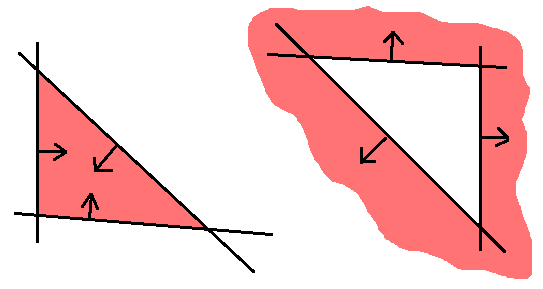
\includegraphics[width=8cm]{graph/shapeinversion}
  \caption[Shape inversion example]{Shape inversion due to the movement of constraints (half-space normals arrows are shown with arrows).}
  \label{fig:shapeinversion}
\end{figure}

\subsubsection{Vertex formulation}
Another possibility was to express the problem in terms of the vertices that form the convex hull of the constraint set.
For this formulation, equation~\ref{eq:arbvolmin} needs to be redefined in terms of the vertices, as shown in equation~\ref{eq:arbvolminverts}
\begin{align}
  \label{eq:arbvolminverts}
    \min_{v}~~&\text{-volume}_{P_i}\\
    \text{s.t.}~~~~ &P_i \subset P_o \notag \\
                    &P_i \text{~and~} P_o \text{~convex} \notag
\end{align}
where $\vect{v}$ is all the vertices of $P_i$.
It needs to be noted that $A$ and $\vect{b}$ will now only result from the final optimized $P_i$.

The vertex based formulation has the following advantages;
\begin{itemize}
  \item This approach is more intuitive as the fitting problem, conceptually, involves moving the vertices of $P_i$ to the facets of $P_o$.
  \item Checking that $P_i$ is inside $P_o$ is now a direct operation, as vertices don't need to be calculated from $A$ and $\vect{b}$ first.
  \item When a measure of containment needs to be generated, consistent gradient information can be expressed in terms of each vertex of $P_i$.
\end{itemize}

Most of the problems with the vertex based method stems from the movement of vertices to the inside of the convex hull of $P_i$ during the solving of the problem.
These internal points are now no longer vertices, but are still considered in the optimization.
This formulation was abandoned in this project due to the following disadvantages in its implementation;
\begin{itemize}
  \item A clear correlation between the number of vertices and the number of facets on a shape does not exist.
Figure~\ref{fig:vertsvsfaces} illustrates this concept for two 6-faceted, 3 dimensional shapes.
This is a major problem when the amount of facets (constraints) on $P_i$ needs to be specified.
  \item A slightly different problem than the one mentioned above -- the number of facets on $P_i$ is determined by the final optimised vertices.
Internal points and duplicate vertices in the solution will cause the number of facets to decrease.
Therefore, specification of a set number of facets becomes nearly impossible.
  \item Enforcing convexity becomes a problem when vertices are used directly.
This is caused by the movement of vertices inside the convex hull of $P_i$.
If all points are to be vertices by definition, non-convex shapes are generated.
The use of the \qhull algorithm to calculate the volume now becomes invalid. 
  \item Another problem with internal points is during the calculation of the volume of $P_i$.
The perturbation of internal points have no effect on the volume (as only the convex hull is considered).
This results in decreased sensitivity of objective functions.
\end{itemize}

\begin{figure}[htbp]
  \centering
  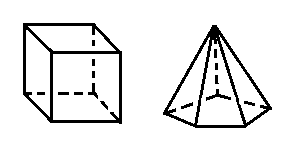
\includegraphics[width=8cm]{graph/vertsvsfaces}
  \caption[The unclear correlation between number of facets and vertices]{A cube and a pentagonal pyramid in 3 dimensions -- both shapes have 6 facets, but differ in their amount of vertices (8 and 6  respectively).}
  \label{fig:vertsvsfaces}
\end{figure}

\subsection{Optimization}
For the solution of the problem, two optimizers/solvers were considered.
Both are contained in the SciPy \texttt{optimize} module;
\begin{itemize}
  \item A sequential least squares quadratic programming (SLSQP) algorithm, \texttt{fmin\_slsqp}, henceforth simply referred to as SLSQP. 
This is a gradient based, constrained solver.
  \item A downhill-simplex algorithm, \texttt{fmin}, henceforth simply referred to as simplex.
This is an unconstrained solver.
\end{itemize}

\subsubsection{Objective functions}
For SLSQP a combination of equality and inequality constraints were used.
The constrained problem formulation for SLSQP is shown in equation~\ref{eq:slsqpobjfn} and follows from equation~\ref{eq:arbvolmin}.
Note that the criteria that $P_i$ should be convex is satisfied by using linear inequalities ($A\vect{x} \leq \vect{b}$) for its construction.
The convexity of $P_o$ is assumed to be a given.
\begin{align}
  \label{eq:slsqpobjfn}
    \min_{A,~\vect{b}}~~&\text{-volume}_{P_i}\\
    \text{s.t.}~~~~ &\text{norm}(\vect{b}) = 1 \notag \\
                    &\text{vertices}_{P_i} \text{~satisfy~} (A\vect{x}\leq\vect{b})_{P_o} \notag  
\end{align}

The constraints as imposed on SLSQP is not possible for simplex.
A penalty formulation for the objective function is therefore used.
Equation~\ref{eq:fminobjfn} shows the objective function for use with simplex.
The same argument for convexity holds as with SLSQP.
\begin{align}
  \label{eq:fminobjfn}
    \min_{A,~\vect{b}}~~&\text{-volume}_{P_i} + p_A(\text{norm}(\text{distance of vertices$_{P_i}$ outside}~P_o)) + p_B(|\text{norm}(\vect{b}) - 1|)  
\end{align}
where $p_A$ and $p_B$ are penalty weights.

The same objective functions (equations~\ref{eq:slsqpobjfn} and~\ref{eq:fminobjfn}) hold for the fitting of rectangular constraint sets.
Only difference begin that $\vect{b}$ is the only input variable and $A$ has a fixed shape (as shown in equation~\ref{eq:recvolmin}).

\subsubsection{Shape exceptions}
Two types of shape exceptions are handled during the optimization.
Firstly, shape inversion (as shown in figure~\ref{fig:shapeinversion}) is handled by giving a sign to the volume.
A sufficient criteria for an open shape is when any one of the vertices violate any one of the constraints used to generate the shape.
If a shape is open, the internal volume is calculated and given a negative sign.

The second class of shape exceptions is that of unbound shapes.
These shapes are generated when enough constraints (used to generate the shape) are parallel, causing the shape to be unbound.
Note that the difference between these open shapes and those resulting from shape inversion is that there are no internal vertices.
In this event, a large bounding $n$-cube is placed around $P_o$, closing the shape but generating vertices that are external to $P_o$.
This method was chosen as opposed to returning an infinite volume.

\subsection{Starting point generation}
For the minimization problem, starting point need to be generated.
A different method for starting point generation is utilized for arbitrary shape fitting and rectangular shape fitting respectively.

Both methods generate a starting shape around the centroid of $P_o$.
With the assumption of convexity the centroid is simply calculated as the average of all the vertices of $P_o$.

For arbitrary shapes, $k-1$ random Gaussian vectors are generated and projected to points on an $n$-sphere (centered around $P_o$'s centroid).
A final vector is generated to ensure a closed shape.
This vector is the negative of the resultant of the first $k-1$ vectors.
Tangential planes to the $n$-sphere at each of the $k$ points are generated.
Finally, the sphere is scaled by a 1\% scaling factor so that the resulting $k$-faceted shape is within $P_o$ (to the largest extent).

For rectangular shapes a deterministic starting point is generated.
An $n$-cube is generated around $P_o$'s centroid.
This cube is then scaled by a 1\% scaling factor to be within $P_o$ (to the largest extent).


%DO THE CODE FOR SURFACE VERTICES AND ADD...


% Local Variables:
% TeX-master: "AHC_thesis"
% End: